%&pdfLaTeX
% !TEX encoding = UTF-8 Unicode

% Nicolás Loira
% 2014

\documentclass{article}

%%%%%%%%%%%%%%%%%%
% INCLUDE

\usepackage[T1]{fontenc}
\usepackage[utf8x]{inputenc}
\usepackage{textcomp}
\usepackage{fullpage}
\usepackage{graphicx}
\usepackage{xspace}
\usepackage{hyperref}

\newcommand{\Meneco}{Meneco$^{++}$\xspace}
\newcommand{\meneco}{meneco$^{++}$\xspace}


\title{\Meneco: philogenetic distance based, gap-filling of metabolic networks}

\author{Nicolas Loira\textsuperscript{1,*},
Sven Thiele\textsuperscript{2},
Santiago Videla\textsuperscript{2},
Sylvain Prigent\textsuperscript{2},\\
Guillaume Collet\textsuperscript{2},
Alejandro Maass\textsuperscript{1,3},
Anne Siegel\textsuperscript{2}\\
{\scriptsize 1 Center for Genome Regulation and Mathomics, Center of Mathematical Modeling, Universidad de Chile.}\\
{\scriptsize 2 Centre Rennes-Bretagne-Atlantique, Projet Dyliss, INRIA, Campus de Beaulieu, 35042 Rennes Cedex, France.}\\
{\scriptsize 3 Department of Mathematical Engineering, Universidad de Chile.} \\
{\scriptsize $*$corresponding author: nloira@dim.uchile.cl}
}

\begin{document}

\maketitle

\section{Abstract}

\begin{itemize}
	\item Metabolic-model reconstruction method produce incomplete networks. Non-functional networks can not be used for predictions. To produce functional networks, extensive manual curation is required.
	\item Gap-filling methods try to find reactions that are missing from the model, in order to fulfill some condition, like biomass production. One of them is Meneco, which provides a list of reactions that may path a non-functional metabolic model.
	\item We improved the meneco method, adding restrictions over the phylogenetic (evolutionary) distance between the organism to be model, and the organisms where the patch reactions are found. In this way, \meneco can find solutions faster, and more accurate than meneco.
	\item We verified the accuracy of our method, removing reactions from a known \emph{E. coli} model, and patching it with reactions from Metacyc. 
\end{itemize}



\section{Introduction}

% REWRITE (from EctoGEM)
MENECO (metabolic network completion), an approach that uses qualitative constraints to test the producibility of a set of metabolites experimentally measured.
This approach is purely qualitative because it studies the topology of a network and the combinatorial interplays between pathways (Schaub and Thiele 2009).

% REWRITE (from EctoGEM)
To address both scalability issues and characteristics of metabolic networks with a high number of reversible reactions and holes, an automatic tool for gap-finding and gap-filling named \meneco was implemented.
This tool analyzes experimental metabolic profiles determined for the species of interest, and suggests reactions to be added to satisfy a topological producibility criterion, thus resulting in a functional metabolic network, i.e. a genome-scale metabolic model.
This method relies on answer set programming (ASP) to efficiently model and solve the gap-filling issue as a combinatorial optimization problem.
ASP is a declarative problem-solving paradigm, in which a problem is encoded as a logic program.
\Meneco deciphers paths that are necessary to produce a set of targeted metabolites identified either by metabolic profiling or by literature-based analysis.
Inputs to the method are: (i) a draft network; (ii) a set of target metabolites that are produced by the organism of interest; (iii) a set of seed nutrients found in the growth media; and (iv) a pool of metabolic reactions available to fill the network (here MetaCyc 17.0).
Following a parsimony principle, \meneco 1.2 reports all minimal sets of candidate reactions in the pool that must be added to the draft network to produce the targets from the seeds.
In addition, \meneco reports the number of unproducible targets before gap-filling, the minimal number of reactions to add to produce the targets and the reactions that are obligatory.

% REWRITE (from EctoGEM)
\Meneco deciphers paths that are necessary to produce a set of targeted metabolites identified either by metabolic profiling or by literature-based analysis.
Inputs to the method are: (i) a draft network; (ii) a set of target metabolites that are produced by the organism of interest; (iii) a set of seed nutrients found in the growth media; and (iv) a pool of metabolic reactions available to fill the network (here MetaCyc 17.0).
Following a parsimony principle, \meneco reports all minimal sets of candidate reactions in the pool that must be added to the draft network to produce the targets from the seeds.
In addition, \meneco reports the number of un-producible targets before gap-filling, the minimal number of reactions to add to produce the targets and the reactions that are obligatory.

Meneco is available at (http://pypi.python.org/pypi/menecopp).



\section{Method}

\Meneco generate a list of possible patches to a metabolic network, in order to fulfill some criteria. A patch is a reaction, taken from a database of reactions, that can be added to a metabolic model. A useful criterion is that the model is functional, that is, that it can produce biomass starting from species available in the media.

Therefore, \meneco can take a metabolic model, a list of seed species (available in the growth media), a list of target metabolites (the biomass requirements), a database of known reactions, and it will produce a set of answers, where each answer will provide a set of reactions that can patch the incomplete model.
To reduce the search space, and provide useful answers, \meneco will give higher priority to reactions that are present in organism phylogenetically close to the modeled organism. To estimate this phylogenetic distance, \meneco will use the distance between 16S genes.


\subsection{ASP based gap-filling}


We address the gap-filling problem by taking advantage of the various reasoning modes provided by ASP. On the one hand, we use ASP’s optimization techniques for finding cardinality or subset minimal solutions, respectively. On the other hand, we exploit consequence aggregation for finding metabolites common to all (optimal) solutions or at least one of them, respectively. Moreover, the aforementioned problems are often subject to additional constraint, aiming at the avoidance of side products or producing target products by staying clear from certain seeds, respectively. Finally, the elaboration tolerance of ASP greatly supports the process of drafting metabolic networks involving continuous validation and increasing functionalities stemming from measured data.


Answer Set Programming. We refer the reader to [6] for a formal introduction to ASP and concentrate in what follows on aspects relevant to our application. A logic program is a finite set of rules of the form...

Logic program representation: Draft Scope, Potential Scope, Metabolic Network Completion, Optimal Completions (plus Sagot semantics), Refined Setting and several Optimization Objectives.




\subsection{Phylogenetic distance}

\Meneco uses the phylogenetic distance between the modeled organism and the organisms associated to the reactions database. Based on these distances, \meneco will look for answer sets that, for example, minimize the phylogenetic distances. A patch of reactions from organisms that are phylogenetically close will be preferred over a patch composed of farther reactions.

As a first step, distance between the modeled organism and the organisms present in the reaction database, should be computed. For our tests, we obtained the 16S sequences for every organism, and then computed a distance based on the BLAST score of the match between each pair of organisms. This distance was discretized to a number from 0 to 5, where 0 is used when no enough information is present, and 1-5 are a measure of distance, 1 being close, 5 being phylogenetically far.

To decide which reactions are better candidates for patching a model, we also need a measure of distance between the modeled organism and each reaction in the database. This distance will be the minimum among the distances from the modeled organism and each of the organism where that reaction is present. In this way, each reaction will have an associated distance to the modeled organism.

\subsection{Optimization strategies}

We defined 4 different optimization objectives for completions: 
minimize the number of reactions (min-card),
subset minimality (min-sub), 
minimize the sum of the reaction scores (min-sum), and  
minimize the maximum score of the reactions (min-max).
We tested different optimization strategies that combine these objectives with different priorities.

\begin{figure}[tb]
	\begin{center}
		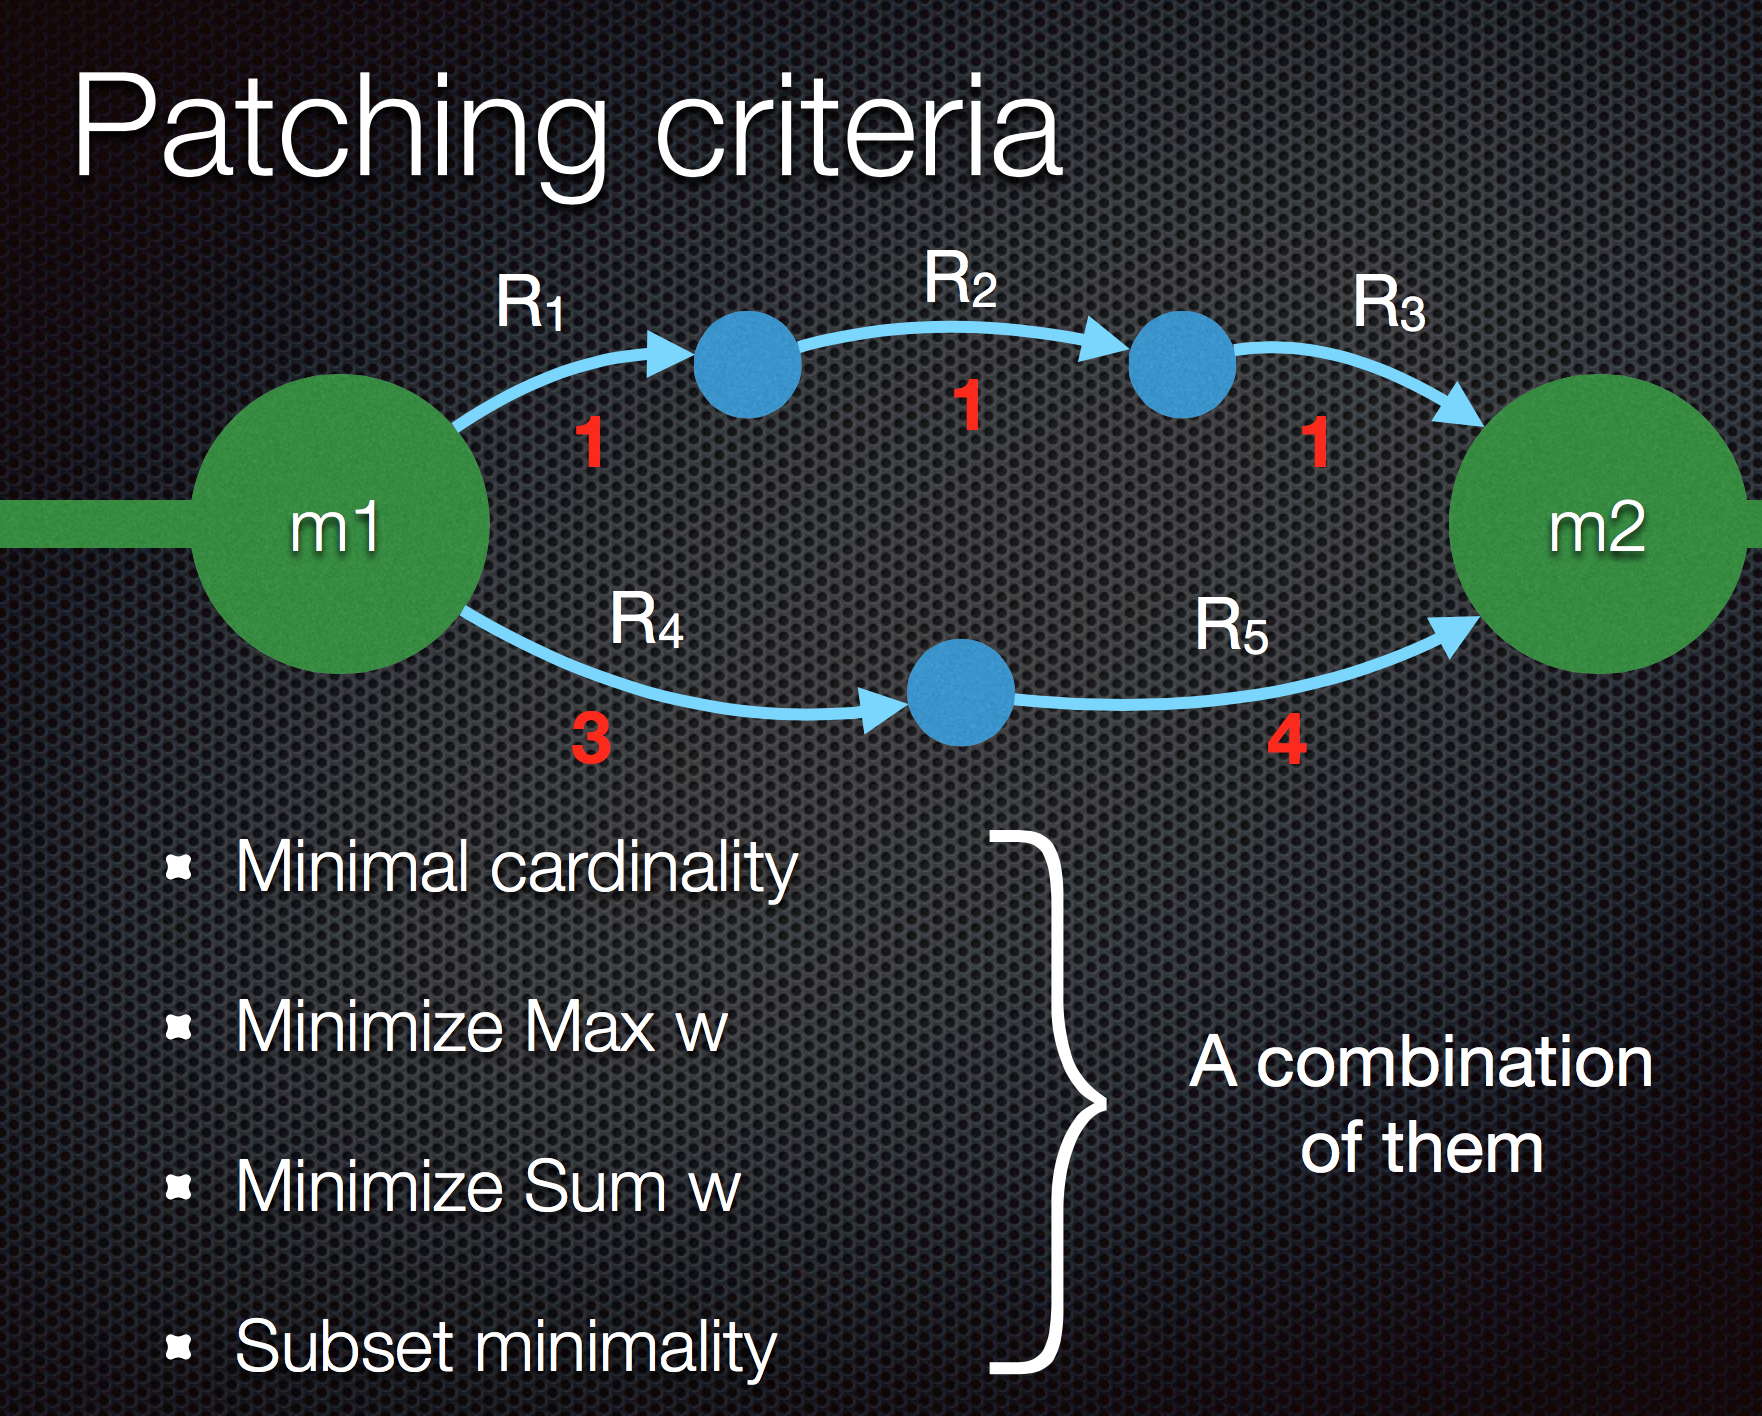
\includegraphics[width=0.5\textwidth]{patchingStrategies.png}
	\end{center}
	\caption[]{The minimal-cardinality strategy will prefer the (R4, R5) patch to complete the model, while the minimal-sum strategy will prefer the longer (R1, R2, R3) patch.}
	\label{fig:figure1}
\end{figure}


\subsection{Bechmark preparation}

\Meneco uses phylogenetic distances to prioritize reactions that are closer to the reconstructed organism. To do this, \meneco needs a measure of that distance. We are trying to build a benchmark, using an incomplete \emph{E. coli} model as the target of reconstruction, and Metacyc as a source of reactions to be used as patches.

During our first try at the benchmark, we used existing databases to obtain the phylogenetic distances between \emph{E. coli} and the rest of the organisms in Metacyc. With this Old Protocol, we covered around 50\% of the needed distances.

Now, instead of using existing distance databases, we developed a New Protocol that computes distances, based on the edit distances between 16S genes.


\subsubsection{Evolutionary distances}

Evolutionary distances will be obtained using the distance provided by the BLAST algorithm, comparing the 16S genes from all of Metacyc's organisms. The steps are:

1. Obtain 16S sequences from the Ribosomal Database Project (RDP). The sequences can be obtained from: \url{http://rdp.cme.msu.edu/misc/resources.jsp}. We used the Unaligned fastas for Bacteria (16S).

2. Translate Metacyc organism names to RDP names:

3. Obtain the 16S sequence for all of Metacyc's organisms:

4. BLAST between the 16S target organism (e.q.: \emph{E. coli}) and the rest of the Metacyc's 16S, in order to obtain a measure of distance.



\section{Result}


\section{Discussion}

\section{References}


\end{document}

